\documentclass[Report.tex]{subfiles}
\externaldocument[I-]{chapter_1_introduction.tex}
\externaldocument[M-]{chapter_2_method.tex}
\externaldocument[D-]{chapter_3_discardMethod.tex}
\externaldocument[C-]{chapter_5_conclusion.tex}
\externaldocument[RE-]{chapter_6_recognition.tex}

\begin{document}
\chapter{Result - Discussion}
\label{chap:Result - Discussion}
\section{Result: Text Segmentation}
We tried 3 Approaches, Morphological, Stroke Width Transform and OpenCv Scene text detection. We end up with the simple solution Morphological approach. It gave good result, but have a lot of limitations. Only work on black text on white paper, image with little noise and only want text in the image. You can see the result in figure \ref{result:fig:Text_seg_result} We could include a part to see if sections of text or non-text. A strategy to do it can be to compare  numbers of connected component, since we know text regions have a lot of letters/component, compare to a coffee cup or a wallet. Canny edge detection can be used to improve it as well. 

\begin{figure}[ht]
  \centering
  \begin{subfigure}[t]{4cm}
    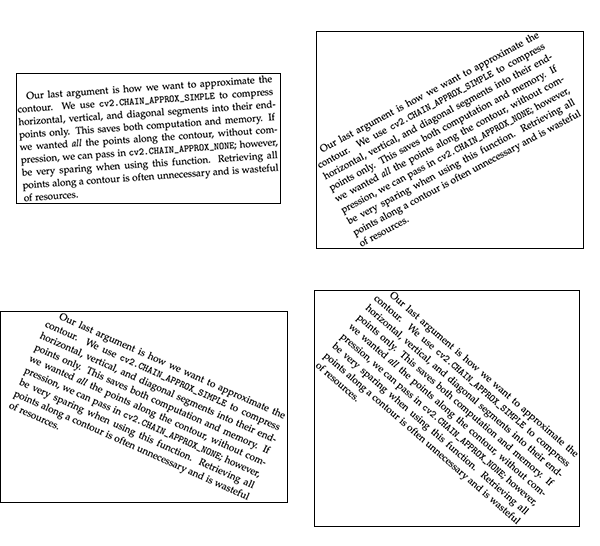
\includegraphics[width=4cm]{res/segment_text1.png}
    \caption{Good result on pure text}
  \end{subfigure}
  \hspace{7mm}%
  \begin{subfigure}[t]{4cm}
    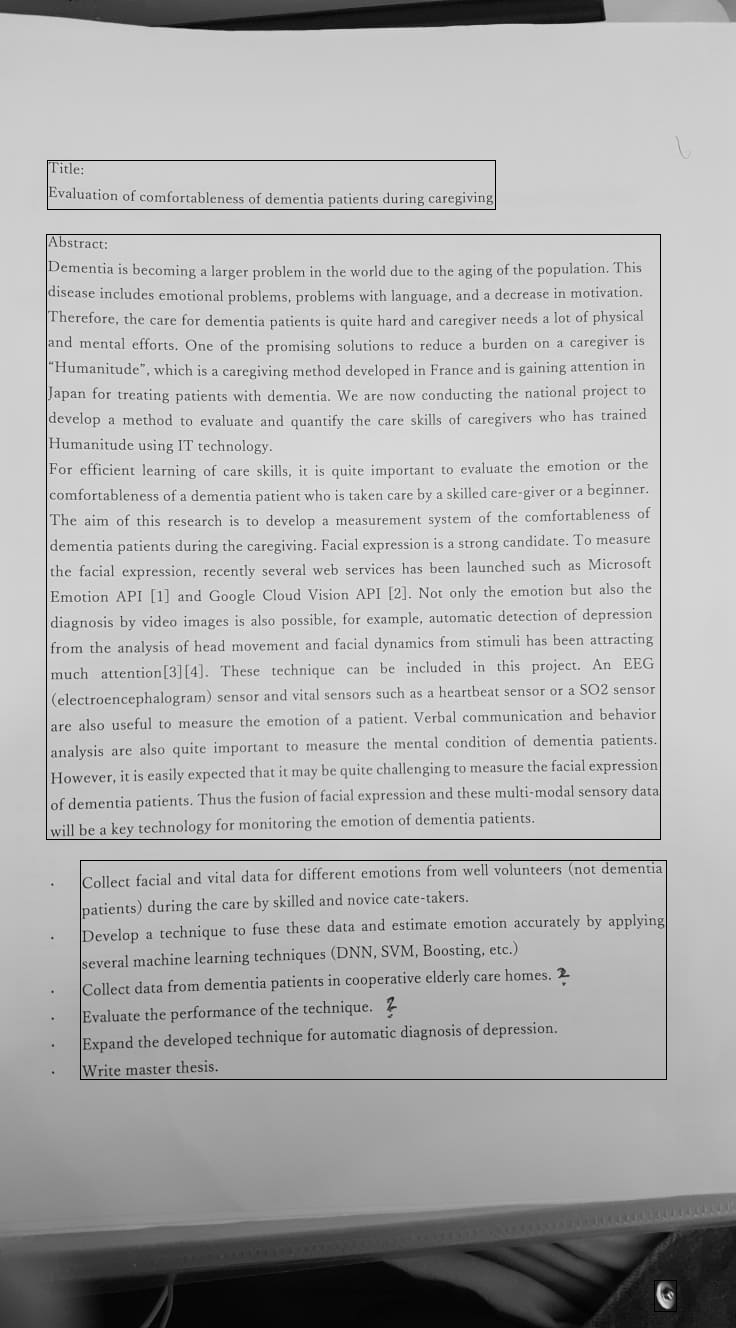
\includegraphics[width=3cm]{res/segment_text2.png}
    \caption{Good result on text on paper with little background noise}
  \end{subfigure}
  \hspace{5mm}%
  \begin{subfigure}[t]{4cm}
    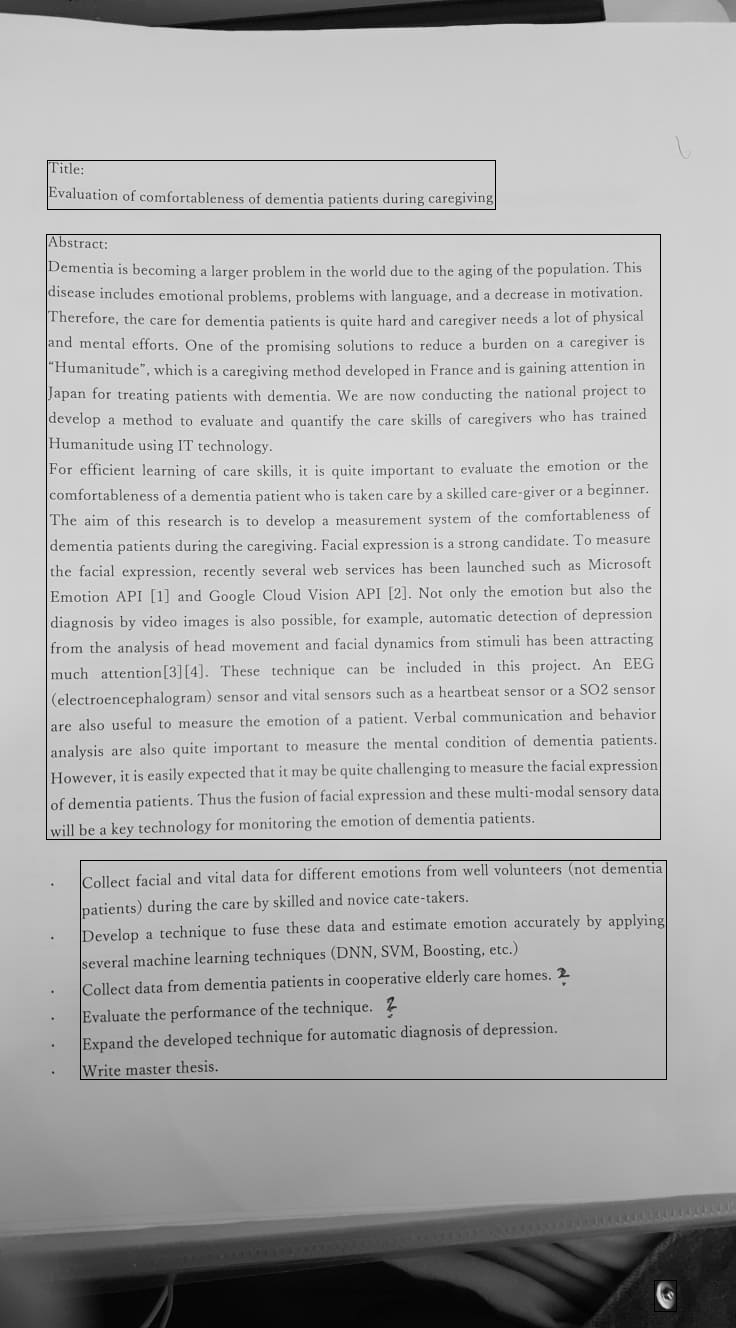
\includegraphics[width=3cm]{res/segment_text3.png}
    \caption{Bad result with many non text object segmented as text}
  \end{subfigure}
  \caption{Result of the Segment Text}
  \label{result:fig:Text_seg_result}
\end{figure}

\section{Result: Preprocessing}

\subsection{Rotation}
Rotation only work if the angle of rotation is less that 45 degree. This problem is mention in section \ref{Method:Preprocessing} and an attempt to solve the problem was given in section \ref{Discard:rotation}. Below are a result image of a less skew image. 

\begin{figure}[ht]
  \centering
  \begin{subfigure}[t]{6cm}
    \frame{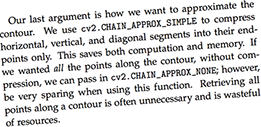
\includegraphics[width=6cm]{res/text_skew_region.png}}
    \caption{Region of skew text, after text segmentation}
  \end{subfigure}
  \hspace{2cm}%
  \begin{subfigure}[t]{6cm}
    \frame{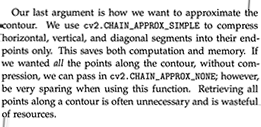
\includegraphics[width=6cm]{res/text_skew_region_rotated.png}}
    \caption{After rotation}
  \end{subfigure}

  \caption{Result of rotation}
  \label{fig:result:rotation}
\end{figure}

\subsection{Line segmentation}
If the image have no space between lines or is slightly skew, it can cause an error, lines will not be separated. Since our previous steps are to handle these problem our method worked quite well on our test images. 
\begin{figure}[ht]
  \centering
  \begin{subfigure}[t]{6cm}
    \frame{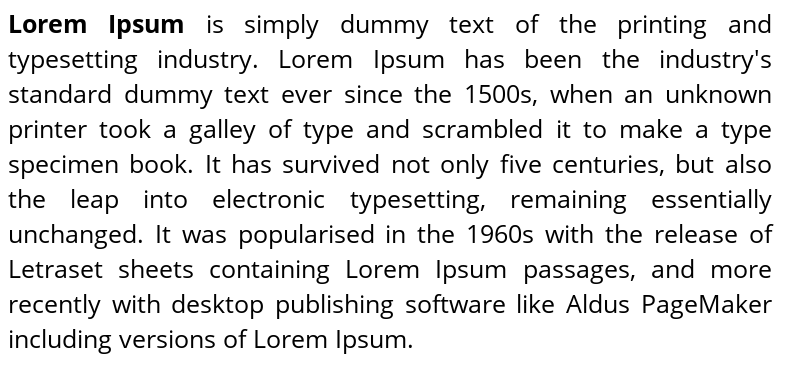
\includegraphics[width=6cm]{res/lorem.png}}
    \caption{Text Region after rotation}
  \end{subfigure}
  \hspace{2cm}%
  \begin{subfigure}[t]{6cm}
    \frame{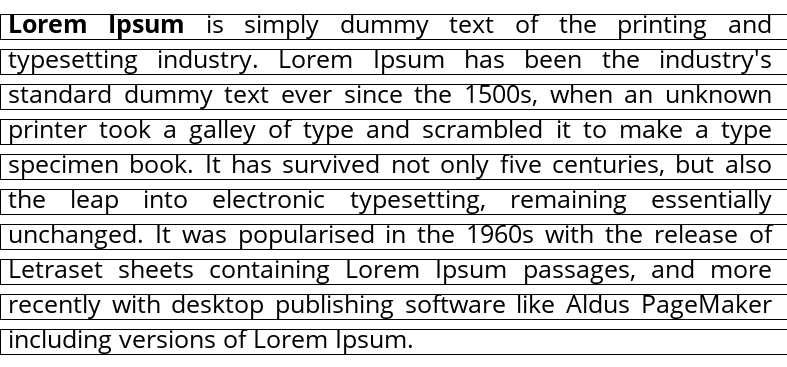
\includegraphics[width=6cm]{res/segment_line.png}}
    \caption{Boundary box of line region}
  \end{subfigure}

  \caption{Result of line segmentation}
  \label{fig:result:rotation}
\end{figure}

\subsection{Character segmentation}
This part worked quiet well, an alternative would be to just using OpenCv findComponent. The steps and result would be much of the same, but we could have dropped cv2.floodFills. A weakness of this approach is if multiple character is merged with one another we would not be able to separate them. A solution for this problem can be to do a morphological opening to separate character better. We did not have test image with that problem, but it came up in latter discussions 

\begin{figure}[H]
  \begin{subfigure}[t]{\textwidth}
    \centering
    
\includegraphics[height=0.45cm]{res/segment_letter1.png}
    \caption{Result of Character Segmentation from extracted line}
  \end{subfigure}
  \begin{subfigure}[t]{\textwidth}
    \centering
    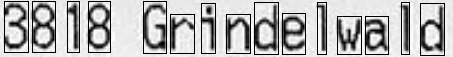
\includegraphics[width=12cm]{res/segment_letter2.png}
    \caption{Result of Character Segmentation from an example line image}
  \end{subfigure}
  \caption{Result of Character segmentation}
  \label{fig:Character_segmentation}
\end{figure}

\section{Result: Classification}
\todo[inline]{Result: Classification}

\subsection{Description}
\begin{flushleft}
  Convolutional neural networks are especially good for image
  classification, because they take local spatial connections into account when
  they classify. This way it doesn't matter where in the image our
  object/character is it will be able to recognize it, same yields for rotation,
  as the CNN classifies based on local spatial connections it doesn't matter if
  the object is rotated. Hence the classification would be even more robust
  compared to the MLP.
\end{flushleft}

\section{Result: Datasets}
\subsection{Description}


\end{document}
